\section{introduction}\label{Sec: intro}
%why data citation
\eat{
In the past few years, we have witnessed rapid increasing amount of information publicly available on line in the form of structured datasets, which requires the curation of domain experts. The curation efforts need recognitions by giving citations to the curated data, which emerges in many scientific domains, such as biological and medical domain. Unlike traditional journal citations with static content and fixed granularity, {\em data citations} vary in the terms of {\em granularity} since different portions of data within a dataset are usually contributed by different groups of people. Data citations are also {\em dynamic} since by the lapse of the time, the appearance of new dataset versions can bring about evolution of the original data citations.}  

The amount of information available online in structured datasets is rapidly increasing, and there is growing interest within both the digital library and computer science communities to be able to cite information extracted by queries over these datasets. Much like a citation to traditional scholarly products such as journal or conference papers, a citation to the result of a query over a structured dataset should include snippets of information describing the dataset (analogous to a title), who is responsible for the dataset (e.g. the PI or contributors/curators of the data), as well as information about how to find the dataset (e.g. the http address, database version, and query). These snippets of information play a significant role in giving credit to those responsible for the data, as well as to enable the data to be reproduced.

%characteristics of data citation
\eat{Typical data citations are generally composed of snippets of information, such as the names of curators (e.g. DBAs or PIs), the curated data (usually represented by a query), the access date and other essential information (e.g. version IDs), which are mostly stored along with the cited data in the database. Those snippets of information in the data citation play a significant role in giving credits to contributors, retrieving the cited data and tracking their versions.}


% Some core principles for data citations are come up with by digital library communities, e.g. CODATA ~\cite{CODATA2013} and FORCE 11~\cite{FORCE11_2104}, which includes some criteria such as 1) \emph{identification and access} to the cited data; 2) \emph{persistence} of the cited data; 3) \emph{completeness} of the reference


%how to construct a data citation
\eat{One example of data citation is the IUPHAR/BPS Guide to Pharmacology~\footnote{http://www.guidetopharmacology.org/} (\iuphar), which is a database of information about drug targets, and the prescription medicines and experimental drugs that act on them. In \iuphar, hard-coded citations are associated with some portions of the data, and include the contributors' names, the query to the cited data, the access date, etc.. It is common to see the coexistence of two type of citations for the same piece of data in \iuphar, i.e. {\em fine-grained citations} for the specific data and {\em coarse-grained citations} for the entire database, which indicates {\em alternative} citations in practice. 
%every target and associated detailed introduction page is edited and developed by a group of contributors whose names are included in hard-coded citations in the corresponding webpages. The citations also include the query to the cited data, the access date, etc..
However, those existing citations fail to meet the increasing demand of requiring the citations to {\em general} queries. Plus, considering a number of applications (e.g. neuro-imaging \cite{HonorEtAl2016}) where users manually pick up the desired tuples for citations from the query instance, it is also essential to construct {\em fine-grained} citations for those selected subsets of query instance.}

One example of how data citation is being implemented is the IUPHAR/BPS Guide to Pharmacology~\footnote{\url{http://www.guidetopharmacology.org/}} (\iuphar), which is a database of information about drug targets, and the prescription medicines and experimental drugs that act on them~\cite{DBLP:journals/nar/SouthanSBFPABDM16}. In \iuphar, citations are associated with certain web-page views of the database, i.e. the data retrieved by certain frequent queries against the database, and are automatically provided along with the query result. This goes well beyond the current practice used by many biomedical databases of providing a traditional journal reference for the database as a whole, and enables credit to be given to the many contributors and curators of different parts of the database.

However, there are some limitations to the approach used in \iuphar.  First, the citations are embedded as SQL queries in the web-pages and cannot be reasoned about independently. Second, since there are a large number of possible queries over a dataset and it is infeasible to specify a citation for each query, there is no way to construct citations to  {\em general} queries, i.e. ones that do not correspond to web-page views.  Third, it does not enable ``fine-grained'' citations.  By this we mean the ability to select a \textit{subset of the query result} and generate a citation to the subset rather than the whole result.  This need  arises in many different scientific applications, in particular neuro-imaging \cite{HonorEtAl2016}. 

%prior work
\eat{
In prior work \cite{wu2018data}\cite{alawini2017automating}\cite{davidson2017model}, we proposed a general framework to {\em automatically} generate \textit{fine-grained} citations for {\em general} queries.
The approach depends on a model of {\em citation views}: {\em Frequent} queries with their existing citations are defined as {\em views} and each snippet of the citations is represented by one {\em citation query}. The formatted citations can be constructed by applying {\em citation functions} over the snippets of information retrieved by {\em citation queries}. For a general query, we can {\em jointly}, {\em alternatively} or {\em aggregately} use the citations of the {\em citation views} to generate citations at various granularities. The interpretations of {\em joint use}, {\em alternative use} and {\em aggregate use} depend on how DBAs choose {\em policies}. \cite{davidson2017model} firstly proposes the concept of {\em citation views}. \cite{alawini2017automating} followed {\em citation views} model and implemented an interactive system called CiteDB and demonstrated how DBAs can define {\em citation views} and {\em policies} in the backend and how users who are not SQL experts execute arbitrary conjunctive queries and obtain citations at various {\em granularities}. \cite{wu2018data} presents the details of three approaches (TLA, SSLA and SLA) that can be utilized by CiteDB and compare their performance by extensive experiments. Among the three approaches, TLA and SSLA are able to reason about {\em fine-grained citations}, which is achieved by explicitly evaluating the satisfiability of the predicates of every view in every query tuple, then determining valid {\em view mappings} and constructing {\em covering sets} for citation generation. The citations for each individual query tuples can be {\em aggregated} to construct citations for arbitrary subsets of query instance and for the entire query. On contrast, SLA can only generate citations at the schema level.  

For a general query, we can {\em jointly}, {\em alternatively} or {\em aggregately} use the citations of the {\em citation views} to generate citations at various granularities. The interpretations of {\em joint use}, {\em alternative use} and {\em aggregate use} depend on how DBAs choose {\em policies}. \cite{davidson2017model} firstly proposes the concept of {\em citation views}. \cite{alawini2017automating} followed {\em citation views} model and implemented an interactive system called CiteDB and demonstrated how DBAs can define {\em citation views} and {\em policies} in the backend and how users who are not SQL experts execute arbitrary conjunctive queries and obtain citations at various {\em granularities}. \cite{wu2018data} presents the details of three approaches (TLA, SSLA and SLA) that can be utilized by CiteDB and compare their performance by extensive experiments. Among the three approaches, TLA and SSLA are able to reason about {\em fine-grained citations}, which is achieved by explicitly evaluating the satisfiability of the predicates of every view in every query tuple, then determining valid {\em view mappings} and constructing {\em covering sets} for citation generation. The citations for each individual query tuples can be {\em aggregated} to construct citations for arbitrary subsets of query instance and for the entire query. On contrast, SLA can only generate citations at the schema level.  
}

In prior work, we proposed a general framework to {\em automatically generate fine-grained citations for general queries} \cite{wu2018data}\cite{alawini2017automating}\cite{davidson2017model}.
  The approach is based on a model of {\em citation views}: Frequent queries  are defined as views with associated citations. A query against the database is rewritten in terms of these views, and the associated citations used to construct a citation for each tuple in the query result. Since a query may be rewritten by \textit{jointly} using more than one view, or there may be several \textit{alternate} ways to rewrite a query, the database owner must specify how citations are jointly or alternatively combined through \textit{policies} (see Figure~\ref{fig:DataCitationFW} for an overview).  The framework also allows for fine-grained citations: the citations for each tuple in the query result are then \textit{combined} to create a final citation for the specified subset of the result, which is given as another policy.  Policies give an interpretation for the joint, alternate and combined use operators, for example, taking the union, intersection or join of the citations.  In the remainder of the paper, we will call this model in \cite{wu2018data} the {\em {\rbafull} (\rba)}.
%\scream{Introduced a shorthand for this so we can change it. Done for the rest of the paper}
%\scream{Need to avoid the word "aggregate" so used "combine" instead.}

%why aggregate queries
As implemented in \cite{wu2018data}, the {\rba} only addresses (non-recursive) conjunctive queries and conjunctive views, and cannot be used in applications in which the queries and views involve aggregates (such as SUM, MIN, AVG) or user-defined functions.  However, there is a growing number of biomedical applications which extract \textit{summaries} from data\-bases by issuing aggregate queries.


One such example is Hetionet, a database that ``encodes'' biology by integrating various types of biological information\eat{about compounds, diseases, genes, anatomies, pathways, biological processes, molecular functions, cellular components, pharmacologic classes, side effects, and symptoms} from different publicly available resources~\cite{himmelstein2017systematic}.
As data is copied from these source datasets, citation information (generally in the form of traditional publication IDs) is also copied and should be propagated to the results of queries.
%and builds connections between them in a Neo4j database. 
\eat{One typical type of citations are the ones indicating a list of publications dedicated to discovering the connections between compounds and genes.
The purpose of Hetionet is to identify patterns of treatment, and predict the probability of treatment among compound-disease pairs \cite{himmelstein2017systematic}.}
\eat{One typical pattern query against this database is one which investigates the biological processes that a certain drug %(e.g. ``Topirmate'') 
affects, and aggregates all the possible ways that this drug binds certain genes, compounds and biological processes. Such pattern queries usually involve aggregation of curation efforts from different people.
In this example, citations for aggregate \textit{queries} are necessary.}
However, the majority of queries involve aggregation over the integrated dataset so the techniques of \cite{wu2018data} cannot be used.

%why aggregate views
Another example, which requires both aggregate queries and aggregate views, is GENCODE~\cite{harrow2012gencode}, an encyclopedia of genes and gene variants whose goal is to identify all functional elements in the human genome using gene annotations. The gene annotation process involves a combination of automatic annotation, manual annotation, and experimental validation. For genes that are manually annotated, information is maintained about the responsible research lab or group. Statistics are also provided for every gene -- an {\em aggregate view} over the genes -- which has another type of citation which gives credit to the creators of the aggregate view.
Common queries over GENCODE also involve aggregation. As an example, one query calculates statistics for every \textit{type} of genes.

\eat{Manual gene annotations come from the Human and Vertebrate Analysis and Annotation (HAVANA) group \footnote{http://www.sanger.ac.uk/research/projects/vertebrategenome/havana/}, while automatic annotations come from Ensembl \cite{flicek2010ensembl}. The two types of annotations are merged, and some are experimentally validated. GENCODE is organized as a hierarchy, with basic information about each gene at the top level, information about exons at the lowest level, and transcripts for gene expression innbetween. %, which are also annotated. 
There exists summary information for every gene and transcript in Ensemble, which specifies whether they are manually or automatically annotated. For those manually annotated ones, HAVANA records which research lab or group in charge of the annotations and citations are essential. GENECODE database also provides statistics for every type of genes which depends on the summary information from Ensemble ({\em views}) and are commonly referenced by the research communities ({\em queries}).}



%why query rewriting using views is not enough since we need fine-grained reasoning
\eat{In order to enable automatic citation generation for aggregate queries, the {\em citation views} model is still utilized, where views can be {\em non-recursive non-nested aggregate views} while the queries are {\em non-recursive non-nested aggregate queries} ({\em aggregate views} and {\em aggregate queries} for short for the rest of paper, which correspond to non-recursive non-nested select-project-join-aggregate SQL queries with possible having clauses). 
% Aggregate views are also common in practice, which usually represents precomputed summary information with citations.
Query rewriting using views algorithms might be a candidate solution to this problem and there have been plenty of them in literatures. However, some limitations of query rewriting using views algorithms prevent its use in data citation. First of all, query rewriting using views algorithms only reason at the schema level for the entire query, which lack the power of {\em fine-grained} reasoning. Plus, to our knowledge, there is no full-fledged query rewriting using views algorithms to be able to deal with the aggregate views with having clauses, which, however, are likely to appear in practice. Among {\em pure view-based approaches} in prior work \cite{wu2018data}, TLA and SSLA can be extended to construct citations for aggregate queries when the views are conjunctive views (details ignored) but cannot handle aggregate views. \cite{wu2018data} and \cite{alawini2018data} point out that data citation is also strongly connected to {\em provenance}. Since the instance of both aggregate queries and aggregate views can be associated with provenance information, which have been thoroughly explored in \cite{amsterdamer2011provenance} and other related work, we turn to applying {\em provenance} to this problem.
}

In this paper, we address the problem of automatically generating fine-grained citations when both the queries and views may involve aggregates.    Although at first glance it would appear that the \rba\ could be extended using results on query writing for aggregate queries~\cite{zaharioudakis2000answering, srivastava1996answering, galindo2001orthogonal,cohen2006rewriting,cohen2006user}, these techniques reason at the schema level for the \textit{entire query result} rather than at the level of individual tuples, which is required for fine-grained citations \scream{Daniel: to discuss. It seems to me that fine-grained and aggregates are orthogonal..}.  Extending the implementation in \cite{wu2018data} to use ideas from query writing for aggregate queries is therefore problematic since aggregates blur the connection between tuples in the input relations and tuples in the result.  Since there is a strong connection between data provenance and data citation, as pointed out in~\cite{alawini2018data}, and the provenance of aggregate queries is well understood~\cite{amsterdamer2011provenance}, we therefore adopt a \textit{\pbafull\ (\pba)}.

\scream{Tova, rephrased.}

\textbf{Example.} (See Figure~\ref{fig:DataCitationFW})  Recall that GENCODE is an encyclopedia of information about genes and gene variants.  Suppose that one of the views defined by the DBA  is $V_{gene}$, which counts the number of genes for each gene type, but only retains the gene types (groups) with more than 10 genes.  This corresponds to an aggregate query with a HA\-VING-clause in SQL.  $V_{gene}$ has an associated citation query which pulls snippets of information from the database and is formatted by the citation function as 
{\tt \{Group: ``Jones Group'', Source: ``HAVANA Project'', ...\}}.

% \begin{tabbing}
% $\lambda G.$\=$V(G, Ty, count(T)) $\hspace{1em}$:-$\=$ Transcript(T, N, Ty', G'), $\\
% \>$Gene(G, N, Ty), G = G', count(T) > 10$
% \end{tabbing}

% This view computes the total number of transcripts for each gene and only the genes with more than 10 transcripts will be retained. 
% Note that if we convert this view query into a SQL query, a having clauses will appear. 
% \begin{tabbing}
% $Q(G, Ty, count(T)) $\hspace{1em}\=$:-$\=$ Transcript(T, N, Ty', G'), $\\
% \>$Gene(G, N, Ty), G = G', Ty = `TEC$'
% \end{tabbing}
Now suppose that a query $Q$ counts the number of genes \textit{whose gene ids are smaller than 50} for every gene type. Then some tuples in the query result will appear in $V_{gene}$, and therefore carry the associated citation.  This is true for the first result tuple in Figure~\ref{fig:DataCitationFW},  where we assume that gene type TEC only include genes whose ids are smaller than 50 and has at least 10 such genes.  Other tuples in the query result may not appear in $V_{gene}$, i.e. gene types which include some genes with ids 50 or greater (which we assume for the second result tuple rRNA)  or which include fewer than 10 genes.  In this case, the tuple would not carry the citation associated with $V_{gene}$.

Traditional query rewriting using views techniques would conclude that $V_{gene}$ is {\em not useful} for $Q$.  Furthermore, the \rba\ tuple-level techniques proposed in~\cite{wu2018data} could not detect whether $V_{gene}$ is useful for a given tuple in the result of $Q$.
However reasoning over the {\em provenance} of result  and view tuples could detect that TEC exists in the view instance (by comparing provenance polynomials) and that all tuples in the group have ids smaller than 50 (by finding the gene ids associated with the provenance tokens).  Thus, if the user in Figure~\ref{fig:DataCitationFW} selects TEC as the subset of interest in the query result, the citation for $V_{gene}$ ({\tt \{Group: "Jones Group", Source: "HAVANA Project", ...\}}) would be returned.
\eat{
in order for a query to be rewritable using a view, one intuition is obeyed by the query rewriting using views algorithms, i.e. under {\em any} database instance $D$, $V_{gene}$ should not eliminate any columns or tuples that are necessary to compute the instance of $Q$, which, however, is violated by $Q$ and $V_{gene}$ in this example because we cannot determine whether all the gene types in the query result exists in the view instance or not since there is a having clause in $V_{gene}$ to filter out gene type with less than 10 genes. But given a specific instance $D$, the existence of a specific gene type in $Q(D)$ (e.g. `TEC') in the view instance and thus whether the query tuple should be associated with the citations from $V_{gene}$ can be determined, which justifies the importance of {\em fine-grained reasoning} in context of data citation and also implies the potential of {\em provenance} to solve this problem since in this example we need to figure out whether ``certain'' view tuple in $V_{gene}(D)$ has type name `TEC'.}
% whether current view instance $V(D)$ retains enough tuples to compute $t_q$ can be determined by {\em provenance}. If there exists one view tuple $t_v$ sharing the same provenance with $t_q$, then it implies that both $t_q$ and $t_v$ originate from the same set of base relation tuples and thus the citations of $t_q$ can be constructed by the citations of $t_v$.
%apply provenance
% Some researchers from digital library domain attempt to enable {\em provenance} property in data citation. For example, Dataverse proposes the use of provenance in data citation in their latest project ``Citation++''\footnote{https://dataverse.org/presentations/citation-data-citation-provenance-and-documentation}. However, Dataverse only generate citations for the entire dataset without providing finer-grained citations. Moreover, it cannot handle automatic citation generation for general queries. 

\textbf{Approach.} Using provenance, we develop a citation system called ProvCite, whose architecture is shown in Figure \ref{fig:DataCitationFW}; the key differences between ProvCite and the \rba\ implementation in~\cite{wu2018data} are indicated by red stars. The system executes over a provenance-enabled relational database system -- here we are using GProM~\cite{arab2018gprom}.
As in \cite{wu2018data}, the DBA defines the citation views and policies to be used.  When a query is submitted, all potential {\em view mappings} are computed, which represent how views can potentially rewrite this query.  The decision of which views are valid, however, depends on the particular result tuple (as illustrated above), and for this the provenance of the result tuple is compared with the provenance of view tuples.  \textit{Covering sets} are calculated from the valid views for each result tuple, representing alternate rewritings in which sets of views are jointly used.  The user is then presented with the query result, and selects the result subset of interest to be cited.  The system finally returns the citations for the selected query tuples. 

\scream{Tova, rephrased.}

Our initial fear in developing ProvCite was that, although the approach is interesting since it develops a novel connection between citation and provenance, it would be unacceptably slow.
That is, the citation should be generated without significantly extending the query time (less than 10 seconds).  However, since the number of possible mappings between the views and the query is exponential in the size of the query, the number and size of the views can be large, the number of result tuples can be large, and provenance expressions are big, this would seem to be an impossible task.  \textit{Surprisingly, the results of this paper not only show that \pba\ is feasible and extends \rba\ results to aggregate queries and views, but that it even outperforms our previous \rba\ approach for aggregate queries and conjunctive views.}

\eat{In order to use provenance for citation reasoning, one {\em provenance system} called ``GProM''\cite{arab2018gprom}\footnote{We are extremely grateful to Boris Glavic for his invaluable support in instructing us to use gprom's source code} is applied to construct the provenance-enable database engine, which retrieve provenance of the query and every view to be used to reason about valid {\em view mapping}s for every query tuples.}
\eat{
Following the same ideas in \cite{wu2018data}, a set of such {\em view mappings} construct {\em covering sets}, each of which represents one single citation. Eventually, Formatted citations, such as JOSN-format citations are generated by applying {\em policies} defined by DBAs, i.e. \{Contributors: Jones Group, Gene Type: `TEC', Query\_id: 101, Source: HAVANA project\}. How {\em covering sets} are constructed from {\em view mappings} and how {formated citations} are produced have been explored in \cite{wu2018data} and will not be repeated here. Instead, how to reason about valid view mappings for each individual tuple level in the context of aggregate queries and  aggregate views becomes our major concerns in this paper.}

\begin{figure}[t!]
    \centering
    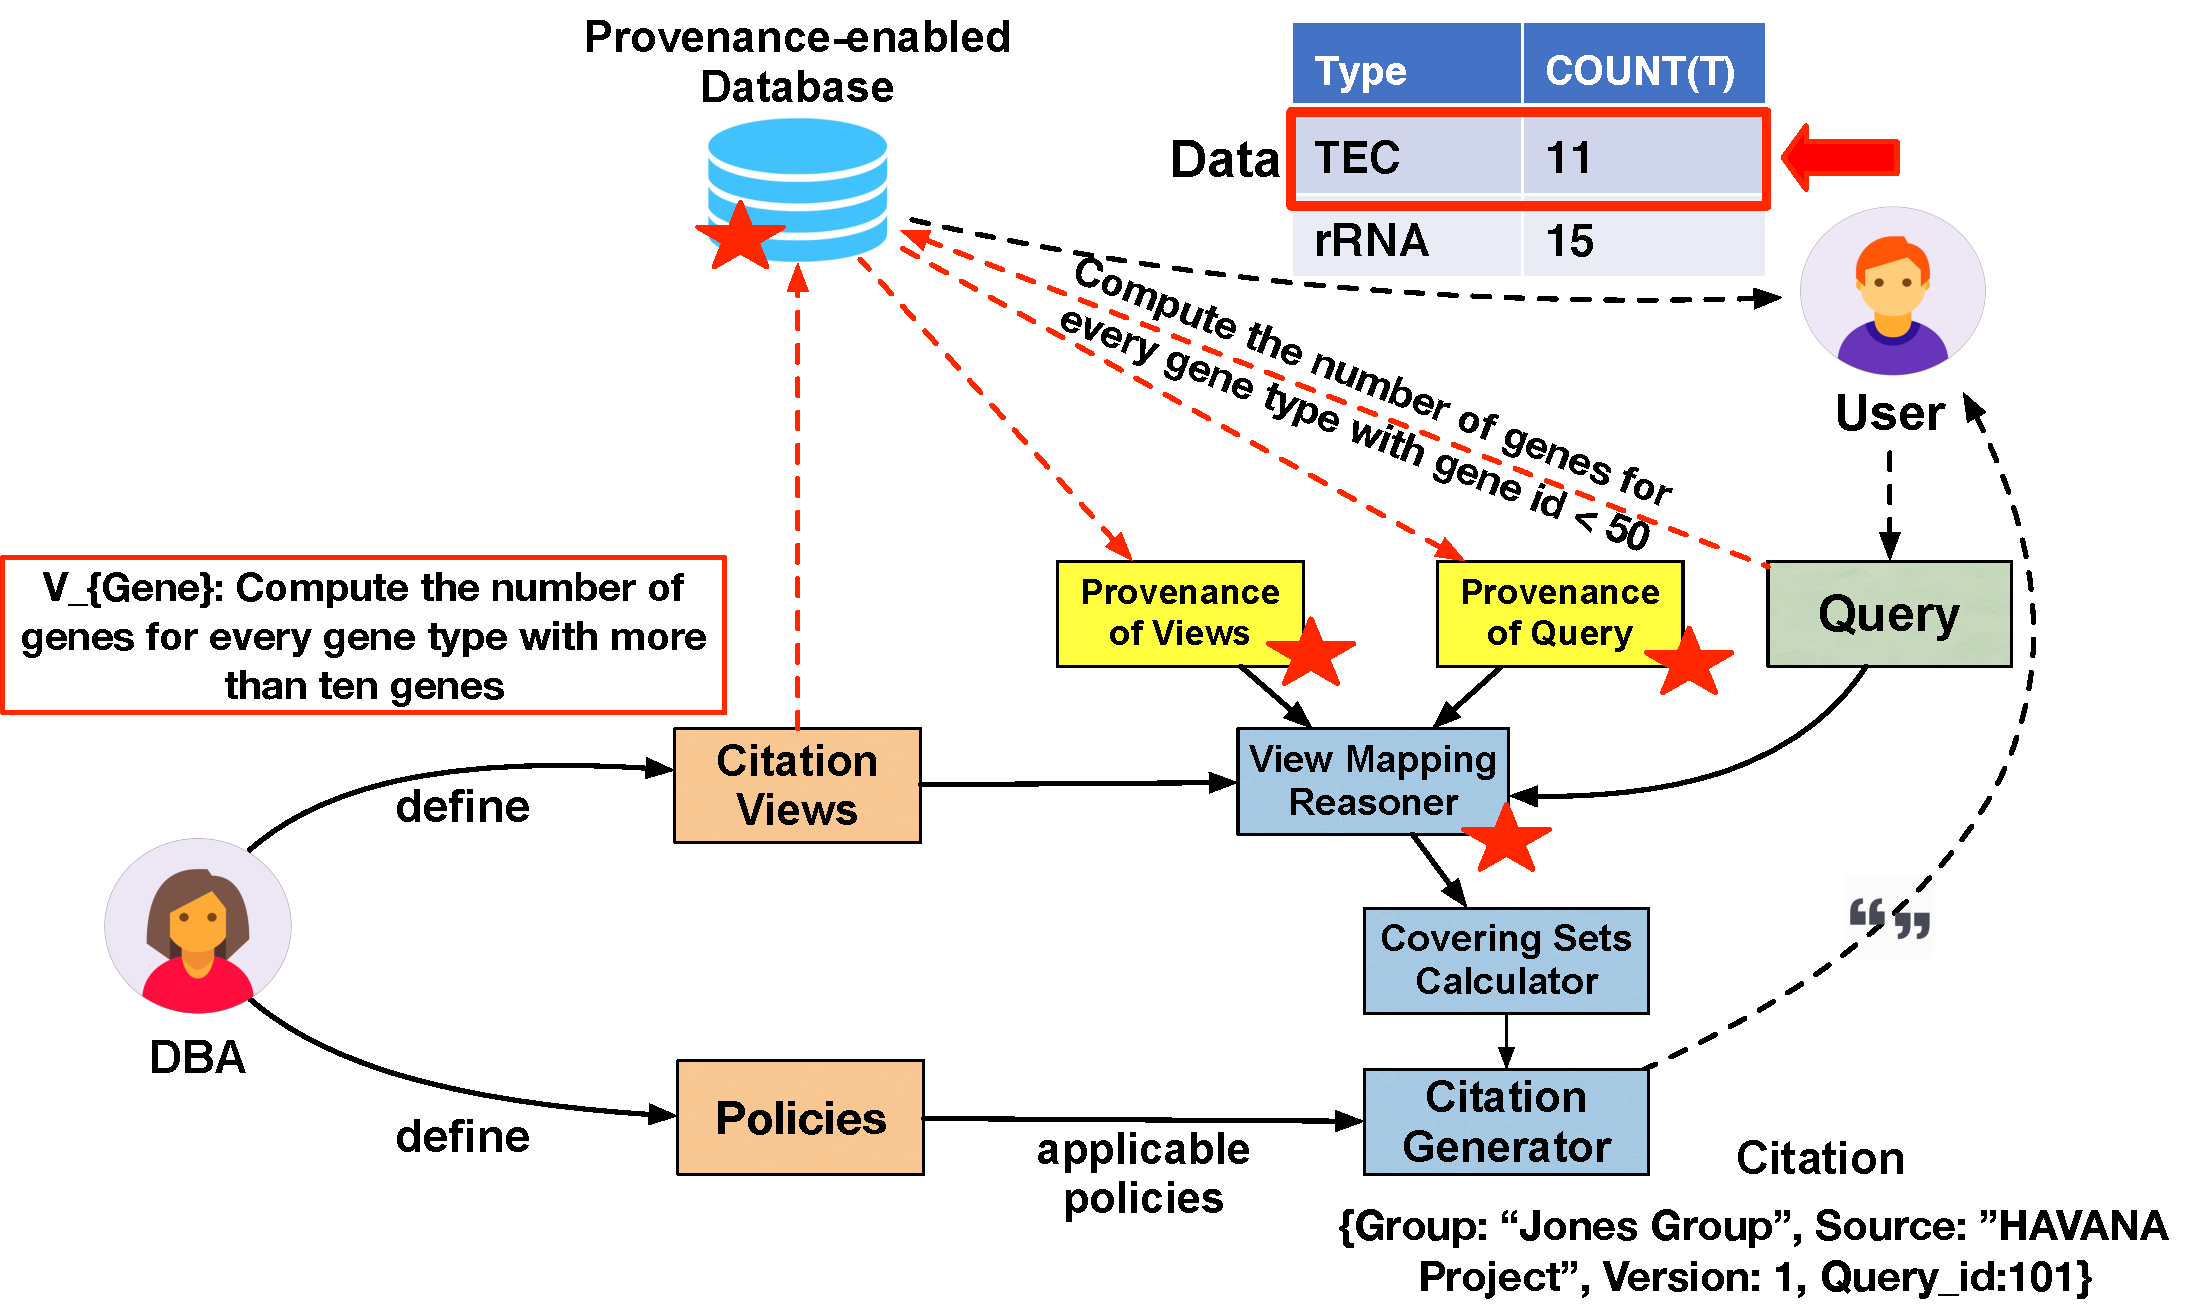
\includegraphics[width=0.48\textwidth,height=0.25\textwidth]{Figures/general_citaiton_framework.pdf}
    \caption{System overview of ProvCite}
    \small \label{fig:DataCitationFW}
\end{figure}

%contributions
{\textbf{Contributions}} of this paper include:

\begin{enumerate}
\item A framework formalizing the connection between data provenance and data citation.
\item %\scream{claim general agg function is supported} 
A semantics for generating citations to the results of aggregate queries with {\em general aggregate functions} given a set of either aggregate or conjunctive views using provenance in the view and query instances.
\item An implementation of the \pba\ called ProvCite, which  automatically generates fine-grained citations for the results of general queries, where both the queries and views may involve aggregates. Two strategies are tested: In the first, provenance is generated on the fly ({\em lazy strategy}), whereas in the second provenance is pre-computed ({\em eager strategy}).
\item 
Experiments using both {\em synthetic}  and {\em realistic} workloads, comparing 
\provalg\ against \rba\ approaches~\cite{wu2018data} in the case of aggregate queries and conjunctive views, and comparing the lazy versus eager strategies for \provalg\ when queries and views involve aggregates.  
\eat{ In {\em synthetic workloads}, the new approach is compared to prior approaches (TLA and SSLA) in the case where all views are $\mathcal{CV}$ while ({\em virtualization strategy}) and ({\em materialization strategy}) are compared to each other in the case where all views are $\mathcal{CAV}$ (which cannot be handled by TLA or SSLA).}
The results show that \provalg\ have acceptable time performance even when the queries and views have large instances, and can in some cases significantly outperform \rba\ approaches.
\eat{feasible in time performance no matter whether the provenance of views are materialized or virtual even when queries and views have large instances; 2) compared to TLA and SSLA, the provenance approach is even about 2x faster than TLA and SSLA in some cases. }
\end{enumerate}

\eat{Yinjun, there are too many sections.  Perhaps fold background information into the model, and/or the algorithm?}
The rest of this paper is organized as follows.
Related work is discussed in Section~\ref{Sec: related_work}, and the running example and preliminaries are given in Section~\ref{Sec: examples}.  Details of the \pba\ and its implementation in ProvCite are presented in Sections~\ref{sec: model} and~\ref{Sec: implementation} respectively. Section~\ref{sec:experiments} gives experimental results before concluding in Section~\ref{sec: conclusion}.


% We have developed a model for automating data citation and implemented three approaches for generating citations at various levels of granularity (tuple level, semi-schema level, and schema level)~\cite{wu2018data}.  The model, however, only works for non-recursive conjunctive queries ($\mathcal{CQ}$) and non-recursive conjunctive views ($\mathcal{CV}$). In this work, we propose a model that uses {\em provenance} to support more complicated queries, i.e. non-recursive select-project-join-aggregate (SPJA) queries ($\mathcal{CAQ}$) and non-recursive select-project-join-aggregate (SPJA) views ($\mathcal{CAV}$). In both $\mathcal{CAQ}$ and $\mathcal{CAV}$, the aggregate operator can only occur as the last step in the query plan (no aggregation in sub-queries), and may have conditions over aggregates (i.e, the HAVING clause)

% In this section, we assume that the form of both the query and views is . 
% To represent such  queries, we use an extended version of Datalog called S-Datalog \cite{consens1990low}, an extension which is commonly used in work on query rewriting using views with aggregation \cite{cohen2006user}\cite{cohen2006rewriting}. In this section, the aggregate operator can only occur as the last step in the query plan (no nesting), and may have conditions over aggregates (i.e, the HAVING clause in SQL) in views and queries, which is not considered in \cite{cohen2006rewriting}.


% \subsection{Why aggregate queries and views}
% In several applications, we have found that users are interested in extracting \textit{summaries} from a database by issuing aggregate queries. 

% Although aggregate queries are common in Hetionet, the citable objects (view queries) are in $\mathcal{CV}$. In this case the reasoning is not very different from the conjunctive query case. 
% We therefore have another example, GENCODE\footnote{www.gencodegenes.org}, where \textit{both the queries and views} are $\mathcal{CAQ}$.  In this case, the reasoning becomes more interesting.

% Since neither of these examples are intuitive, in the paper (to be written) we will develop complex queries and views using a database of computer science publications (extracted from DBLP) and funding sources (extracted from the NSF website).  We will mention, but not build on, the use cases of Hetionet, IUPHAR and GENCODE.
